\item \subquestionpointscodingandwritten{4} {\bf Degree-$k$ polynomial regression}

Now we extend the idea above to degree-$k$ polynomials by considering $\phi:\mathbb{R}\rightarrow \mathbb{R}^{k+1}$ to be 
		\begin{align}
	\phi(x) = \left[\begin{array}{c} 1\\ x \\ x^2\\ \vdots \\x^k \end{array}\right]\in \mathbb{R}^{k+1} \label{eqn:feature-k}
	\end{align}

Follow the same procedure as the previous sub-question, and implement the algorithm with $k=1,2,3,5,10,20$. To verify a correct implementation, consider creating a similar plot as in the previous sub-question, and include the the hypothesis curves for each value of $k$ with a different color. Include a legend in the plot to indicate which color is for which value of $k$.  Briefly comment on your observations of the fit for each K value (below).  This plot should look similar to the following:
\begin{figure}[H]
  \centering
  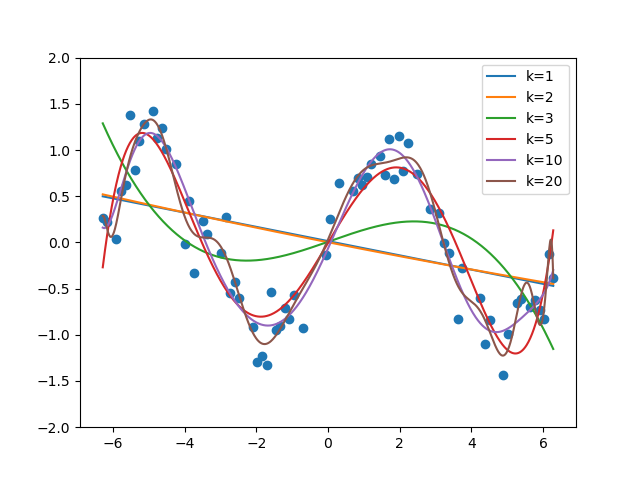
\includegraphics[width=0.65\linewidth]{featuremaps/src/large-poly.png}
  \centering
\caption{Polynomial regression with kernel sizes 1,2,3,5,10 and 20}
\end{figure}

Provide your explanation of the fit for each K value here:

\hl{We created degree-k polynomial features from our original dataset. From the plot, we see that k=5,10,20 are very similar to one another and follows the scattered data points well. This is because the feature $x^4$ is a good feature for the training data. What we see in the plot is that once $k>=4$, $x^4$ becomes available and is given a big $\theta$ for the model.}
\\[50pt]